%%%%%%%%%%%%%%%%%%%%%%%%%%%%%%%%%%%%%%%%%%%%%%%%%%%%%%%%%%%%%%%%%%%%%%%%%%%%%%%%%%%%%%%%%%%%%%%%%%%%%%%%%%%%%%%%%%%%%%%%%%%%%%%%%%%%%%%%%%%%%%%%%%%%%%%%%%%%%%%%%%%
% Written By Michael Brodskiy
% Class: Analysis of Random Phenomena
% Professor: I. Salama
%%%%%%%%%%%%%%%%%%%%%%%%%%%%%%%%%%%%%%%%%%%%%%%%%%%%%%%%%%%%%%%%%%%%%%%%%%%%%%%%%%%%%%%%%%%%%%%%%%%%%%%%%%%%%%%%%%%%%%%%%%%%%%%%%%%%%%%%%%%%%%%%%%%%%%%%%%%%%%%%%%%

\include{Includes.tex}

\title{Homework 8}
\date{\today}
\author{Michael Brodskiy\\ \small Professor: I. Salama}

\begin{document}

\maketitle

\begin{enumerate}

  \item We may write the correlation coefficient as:

    $$\rho_{XY}=\frac{\text{Cov}(X,Y)}{\sqrt{\text{Var}(X)\text{Var}(Y)}}$$

    Given that $Y=X+2Z$, we obtain:

    $$\text{Cov}(X,Y)=\text{Cov}(X,X+2Z)$$

    We break this apart to get:

    $$\text{Cov}(X,X+2Z)=\text{Cov}(X,X)+2\text{Cov}(X,Z)$$
    $$\text{Cov}(X,X+2Z)=\text{Var}(X)+2\text{Cov}(X,Z)$$

    Additionally, we get:

    $$\text{Var}(Y)=\text{Var}(X+2Z)$$
    $$\text{Var}(X+2Z)=\text{Var}(X)+4\text{Var}(Z)+4\text{Cov}(X,Z)$$

    Thus, the expression becomes:

    $$\rho_{XY}=\frac{\text{Var}(X)+2\text{Cov}(X,Z)}{\sqrt{\text{Var}(X)[\text{Var}(X)+4\text{Var}(Z)+4\text{Cov}(X,Z)]}}$$

    The final step is to calculate the covariance between $X$ and $Z$. Since it is stated that the two are independent, we arrive at:

    $$\text{Cov}(X,Z)=0$$

    And thus:

    $$\rho_{XY}=\frac{\text{Var}(X)}{\sqrt{\text{Var}(X)[\text{Var}(X)+4\text{Var}(Z)]}}$$

    We plug in our known values to get:

    $$\rho_{XY}=\frac{16}{\sqrt{16[(16)+4(4)]}}$$
    $$\boxed{\rho_{XY}=\frac{\sqrt{2}}{2}}$$

    Since the correlation coefficient is not zero, \underline{$X$ and $Y$ are not independent}.

    Now, given $W=2X-Z$, we want to find:

    $$E[W]=E[2X-Z]$$
    $$\text{Var}(W)=\text{Var}(2X-Z)$$
    $$\text{Cov}(W,Y)=\text{Cov}(2X-Z,X+2Z)$$

    For the expectation value, we simply decompose to get:

    $$E[W]=2E[X]-E[Z]$$
    $$E[W]=2(2)-1$$
    $$\boxed{E[W]=3}$$

    The variance can be expanded to get:

    $$\text{Var}(W)=4\text{Var}(X)+\text{Var}(Z)-4\cancel{\text{Cov}(X,Z)}$$
    $$\text{Var}(W)=4(16)+4$$
    $$\boxed{\text{Var}(W)=68}$$

    Finally, we find the covariance as:

    $$\text{Cov}(W,Y)=\text{Cov}(2X,X+2Z)-\text{Cov}(Z, X+2Z)$$
    $$\text{Cov}(W,Y)=2\text{Var}(X) + 3\text{Cov}(X,Z)-2\text{Var}(Z)$$

    Plugging in values, we get:

    $$\text{Cov}(W,Y)=2(16) + \cancel{3\text{Cov}(X,Z)}-2(4)$$
    $$\boxed{\text{Cov}(W,Y)=24}$$

  \item

    \begin{enumerate}

      \item We may begin by expressing $E[Y]$ as:

        $$E[Y]=2E[X_1]-E[X_2^2]$$

        This gives us:

        $$E[Y]=2(0)-\int_{-1.5}^{1.5} \frac{x^2}{3}\,dx$$
        $$E[Y]=-\frac{x^3}{9}\Big|_{-1.5}^{1.5}$$
        $$\boxed{E[Y]=-\frac{3}{4}}$$

      \item Similarly, we separate the variance to get:

        $$\text{Var}(Y)=4\text{Var}(X_1)+\text{Var}(X_2^2)$$

        Using our standard uniform formula, we find:

        $$\text{Var}(X_1)=\frac{(3)^2}{12}$$
        $$\text{Var}(X_1)=\frac{3}{4}$$

        We can then express $\text{Var}(X_2^2)$ as:

        $$\text{Var}(X^2_2)=E[X_2^4]-E[X_2^2]^2$$

        We compute this and enter already calculated values to get:

        $$\text{Var}(X^2_2)=\int_{-1.5}^{1.5}\frac{x^4}{3}\,dx-(.75)^2$$
        $$\text{Var}(X^2_2)=\frac{x^5}{15}\Big|_{-1.5}^{1.5}-(.75)^2$$
        $$\text{Var}(X^2_2)=1.0125-.5625$$
        $$\text{Var}(X^2_2)=.45$$

        We sum to get:

        $$\text{Var}(Y)=4(.75)+.45$$
        $$\boxed{\text{Var}(Y)=3.45}$$

      \item Finally, we can calculate the covariance as:

        $$\text{Cov}(Y,X_1)=\text{Cov}(2X_1-X_2^2,X_1)$$

        We expand to get:

        $$\text{Cov}(2X_1-X_2^2,X_1)=2\text{Var}(X_1)-\text{Cov}(X_2^2,X_1)$$

        Given that $X_2$ and $X_1$ are independent, the covariance term becomes zero and we get:

        $$\text{Cov}(Y,X_1)=2\text{Var}(X_1)$$
        $$\text{Cov}(Y,X_1)=2(.75)$$
        $$\boxed{\text{Cov}(Y,X_1)=1.5}$$

    \end{enumerate}

  \item

    \begin{enumerate}

      \item To find the joint PDF, we may use the following formula:

        $$f_{XY}(x,y)=\frac{1}{\sqrt{2\pi(1-\rho^2)\sigma_x\sigma_y}}e^{-\frac{1}{2}\left[ \frac{(x-\mu_x)^2}{\sigma_x^2}-2\rho\left( \frac{x-\mu_x}{\sigma_x} \right)\left( \frac{y-\mu_y}{\sigma_y} \right)+\frac{(y-\mu_y)^2}{\sigma_y^2}  \right]}$$

        We enter our given values to get:

        $$f_{XY}(x,y)=\frac{1}{\sqrt{2\pi(1-.25)(4)(2)}}e^{-\frac{1}{2}\left[ \frac{(x-1)^2}{16}-\left( \frac{x-1}{4} \right)\left( \frac{y-2}{2} \right)+\frac{(y-2)^2}{4}  \right]}$$
        $$\boxed{f_{XY}(x,y)=\frac{1}{\sqrt{12\pi}}e^{-\frac{1}{2}\left[ \frac{(x-1)^2}{16}-\left( \frac{x-1}{4} \right)\left( \frac{y-2}{2} \right)+\frac{(y-2)^2}{4}  \right]}}$$

      \item Given $V=2X-3Y$, we may write:

        $$E[V]=E[2X-3Y]$$
        $$\text{Var}(V)=\text{Var}(2X-3Y)$$

        We can obtain the former by writing:

        $$E[V]=2E[X]-3E[Y]$$
        $$E[V]=2(1)-3(2)$$
        $$\boxed{E[V]=-4}$$

        Similarly, we expand the variance to write:

        $$\text{Var}(V)=4\text{Var}(X)+9\text{Var}(Y)-12\text{Cov}(X,Y)$$
        $$\text{Var}(V)=4\text{Var}(X)+9\text{Var}(Y)-12\rho_{XY}\sigma_x\sigma_y$$
        $$\text{Var}(V)=4(4)^2+9(2)^2-12\left( \frac{1}{2} \right)\left( 4 \right)\left( 2 \right)$$
        $$\text{Var}(V)=64+36-48$$
        $$\boxed{\text{Var}(V)=52}$$

      \item Since we know that a linear combination of normal variables also yields a normal variable, we can write:

        $$V=\text{Norm}(-4, 52)$$

        Accordingly, we find:

        $$P[V>4]=1-P\left[ \frac{V-\mu_v}{\sigma_v} \leq \frac{4-\mu_v}{\sigma_v} \right]$$

        This gives us:

        $$P[V>4]=1-P\left[ Z \leq 1.1094 \right]$$
        $$\boxed{P[V>4]=.1336}$$

    \end{enumerate}

  \item We may begin by finding the marginal PDF of $X$:

    $$f_X(x)=\int_0^{2x} 1\,dy$$
    $$f_X(x)=2x,\quad 0\leq x\leq 1$$

    We can then find the expected value as:

    $$E[X]=\int_0^1 2x^2\,dx$$
    $$E[X]=\frac{2}{3}x^3\Big|_0^1$$
    $$E[X]=\frac{2}{3}$$

    From here, we find the variance as:

    $$\text{Var}(X)=\int_{0}^1 \left( x-\frac{2}{3} \right)^2 (2x)\,dx$$
    $$\boxed{\text{Var}(X)=\frac{1}{18}}$$

    Similarly, we may find the marginal PDF of $y$ as:

    $$f_Y(y)=\int_{y/2}^1 1\,dx$$
    $$f_Y(y)=1-\frac{y}{2},\quad 0\leq y\leq 2$$

    We then find the expectation value as:

    $$E[Y]=\int_0^2 y\left( 1-\frac{y}{2} \right)\,dy$$
    $$E[Y]=\int_0^2 y-\frac{y^2}{2}\,dy$$
    $$E[Y]=\frac{y^2}{2}-\frac{y^3}{6}\Big|_0^2$$
    $$E[Y]=\frac{2}{3}$$

    We then find the variance as:

    $$\text{Var}(Y)=\int_0^2 \left( y-\frac{2}{3} \right)^2\left( 1-\frac{y}{2} \right)\,dy$$
    $$\boxed{\text{Var}(Y)=\frac{2}{9}}$$

    Then, to compute the covariance, we obtain:

    $$E[XY]=\int_0^1\int_0^{2x} xy\,dy\,dx$$

    This gives us:

    $$E[XY]=\left( \frac{x^4}{2} \right)\Big|_0^1$$
    $$E[XY]=\frac{1}{2}$$

    This leads to the covariance as:

    $$\text{Cov}(X,Y)=\frac{1}{2}-\left( \frac{2}{3} \right)\left( \frac{2}{3} \right)$$
    $$\boxed{\text{Cov}(X,Y)=\frac{1}{18}}$$

    We then use the above calculated values to find the total packet variance, or:

    $$\text{Var}(X+Y)=\text{Var}(X)+\text{Var}(Y)+2\text{Cov}(X,Y)$$

    Entering our known values, we get:

    $$\text{Var}(X+Y)=\frac{1}{18}+\frac{2}{9}+2\left( \frac{1}{18} \right)$$
    $$\boxed{\text{Var}(X+Y)=\frac{7}{18}}$$

  \item

    \begin{enumerate}

      \item We may observe that, based on the given information, the Null Hypothesis may be written as:

        $$\boxed{H_o: p=.2\quad\text{(failure rate remains .2)}}$$

        Furthermore, the alternative hypothesis becomes:

        $\boxed{H_1: p<.2\quad\text{(failure rate is below .2)}}$

      \item Given a fixed number of trials, we may observe that the number of failures must follow a binomial distribution. We may write this as:

        $$X=\text{Binomial}(20,.2)$$

        We may expand this for $H_o$ to write:

        $$\boxed{P[X=k]=\left( \begin{matrix} 20\\k\end{matrix} \right).2^k.8^{20-k}}$$

        For $H_1$, the distribution shifts since the probability would be below $p=.2$, meaning that $p$ decreases and $1-p$ increases.

      \item We know that our expectation value may be written as:

        $$E[X|H_o]=np$$
        $$E[X|H_o]=(20)(.2)$$
        $$\boxed{E[X|H_o]=4\text{ failures}}$$

      \item There are two types of errors we may observe:

        \begin{itemize}

          \item Type I Error, labeled $\alpha$ — This occurs when the null hypothesis is rejected despite being true. Given this problem, we would find that the probability of failure is \underline{not} $p=.2$, despite the error rate actually being $p=.2$

          \item Type II Error, labeled $\beta$ — This occurs when the null hypothesis is not rejected, despite being false. In this case, we would find that the error rate probability is $p=.2$, even though the actual failure rate is less.

        \end{itemize}

      \item We are given a threshold to reject $H_o$ if $X\leq 1$, and accept $H_o$ if $X>1$. Accordingly, a Type I Error ($\alpha$) will occur with probability:

        $$\alpha = P[X=1]+P[X=0]$$
        $$\alpha = .057646+.011529$$
        $$\boxed{\alpha = .069175}$$

      \item Making a Type II Error would mean that the actual probability is $p=.1$, but we find the $p=.2$. This means that the probability of making a Type II Error is the probability of the null hypothesis being accepted with $p=.2$. We can write a $z$-score as:

        $$z=\frac{.2-.1}{4(.8)/\sqrt{20}}$$
        $$z=.25$$

        Then taking an inverse CDF function, we find:

        $$\beta=\text{invCDF}(.25)$$
        $$\boxed{\beta=.4013}$$

        The power is thus:

        $$\text{Power}=1-\beta$$
        $$\boxed{\text{Power}=.5987}$$

      \item Since we are required to keep the sample size and difference between probabilities constant, our only option to increase the power is to increase the significance value, $\alpha$. We can check our $\alpha$ value from (e) to get:

        $$Z=\text{invCDF}\left(1-\frac{\alpha}{2}\right)$$
        $$Z=\text{invCDF}(.9654)$$
        $$Z=1.8171$$

        We then use this $z$-score to obtain:

        $$\bar{x}=.2-1.8171\left( \frac{1.7889}{\sqrt{20}} \right)$$
        $$\bar{x}=-.5269$$

        We then find the $\beta$ value by using:

        $$P\left[ Z\geq \frac{-.5269-.1}{1.7889\sqrt{20}} \right]$$
        $$P\left[ Z\geq -.078355 \right]=\beta$$
        $$\boxed{\beta=.4688}$$

        Thus, we may see that we are not using an adequate $\alpha$ value for enough power.

    \end{enumerate}

    \setcounter{enumi}{4}

  \item \textbf{Extra Credit}

    \begin{enumerate}

      \item The tree diagram can be drawn as:

        \begin{figure}[H]
          \centering
          \tikzset{every picture/.style={line width=0.75pt}} %set default line width to 0.75pt        

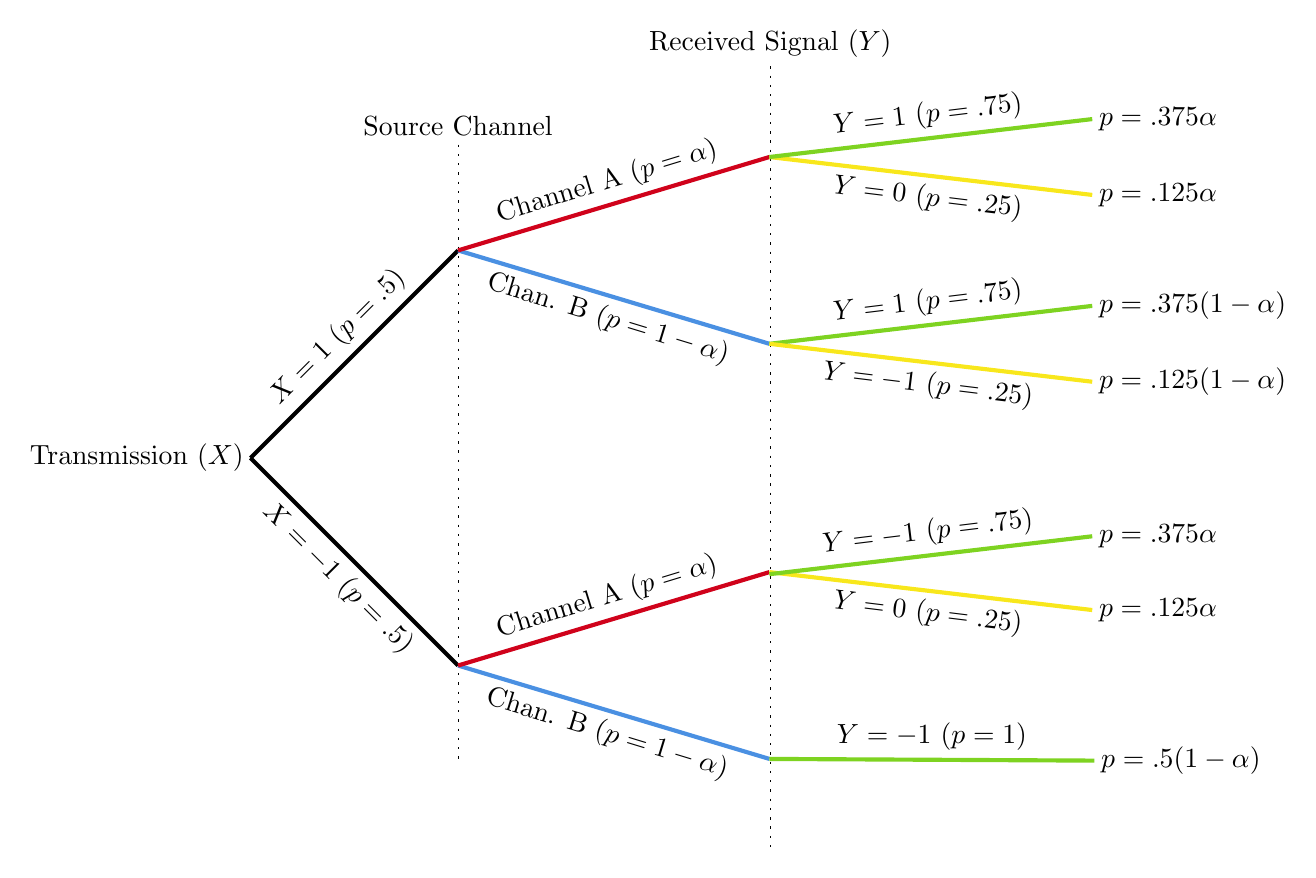
\begin{tikzpicture}[x=0.75pt,y=0.75pt,yscale=-1,xscale=1]
%uncomment if require: \path (0,493); %set diagram left start at 0, and has height of 493

%Straight Lines [id:da23791128150940755] 
\draw [line width=1.5]    (124,251) -- (224,151) ;
%Straight Lines [id:da3966057563521548] 
\draw [line width=1.5]    (124,251) -- (224,351) ;
%Straight Lines [id:da915484597228999] 
\draw  [dash pattern={on 0.84pt off 2.51pt}]  (224,100) -- (224,396.42) ;
%Straight Lines [id:da1241748882024809] 
\draw [color={rgb, 255:red, 74; green, 144; blue, 226 }  ,draw opacity=1 ][line width=1.5]    (224,151) -- (374,196) ;
%Straight Lines [id:da5569456827980495] 
\draw [color={rgb, 255:red, 208; green, 2; blue, 27 }  ,draw opacity=1 ][line width=1.5]    (374,106) -- (224,151) ;
%Straight Lines [id:da011409041725653823] 
\draw [color={rgb, 255:red, 74; green, 144; blue, 226 }  ,draw opacity=1 ][line width=1.5]    (224,351) -- (374,396) ;
%Straight Lines [id:da8043679678690399] 
\draw [color={rgb, 255:red, 208; green, 2; blue, 27 }  ,draw opacity=1 ][line width=1.5]    (374,306) -- (224,351) ;
%Straight Lines [id:da9802980049289851] 
\draw  [dash pattern={on 0.84pt off 2.51pt}]  (374.42,62.29) -- (374.42,439.71) ;
%Straight Lines [id:da4884123484523494] 
\draw [color={rgb, 255:red, 248; green, 231; blue, 28 }  ,draw opacity=1 ][line width=1.5]    (374,106) -- (529.54,124.27) ;
%Straight Lines [id:da12971510506081663] 
\draw [color={rgb, 255:red, 126; green, 211; blue, 33 }  ,draw opacity=1 ][line width=1.5]    (529.54,177.73) -- (374,196) ;
%Straight Lines [id:da7130390548310087] 
\draw [color={rgb, 255:red, 126; green, 211; blue, 33 }  ,draw opacity=1 ][line width=1.5]    (529.54,87.73) -- (374,106) ;
%Straight Lines [id:da7886014049297126] 
\draw [color={rgb, 255:red, 248; green, 231; blue, 28 }  ,draw opacity=1 ][line width=1.5]    (374,196) -- (529.54,214.27) ;
%Straight Lines [id:da8437771671847172] 
\draw [color={rgb, 255:red, 248; green, 231; blue, 28 }  ,draw opacity=1 ][line width=1.5]    (374,306) -- (529.54,324.27) ;
%Straight Lines [id:da4450873514693551] 
\draw [color={rgb, 255:red, 126; green, 211; blue, 33 }  ,draw opacity=1 ][line width=1.5]    (529.54,288.73) -- (374,307) ;
%Straight Lines [id:da04003805736905319] 
\draw [color={rgb, 255:red, 126; green, 211; blue, 33 }  ,draw opacity=1 ][line width=1.5]    (530.6,396.82) -- (374,396) ;

% Text Node
\draw (171.6,198.6) node [anchor=south] [inner sep=0.75pt]  [rotate=-315]  {$X=1\ ( p=.5)$};
% Text Node
\draw (171.6,303.4) node [anchor=north] [inner sep=0.75pt]  [rotate=-45]  {$X=-1\ ( p=.5)$};
% Text Node
\draw (122,251) node [anchor=east] [inner sep=0.75pt]   [align=left] {Transmission ($\displaystyle X$)};
% Text Node
\draw (224,97) node [anchor=south] [inner sep=0.75pt]   [align=left] {Source Channel};
% Text Node
\draw (298.12,125.63) node [anchor=south] [inner sep=0.75pt]  [rotate=-343] [align=left] {Channel A ($\displaystyle p=\alpha $)};
% Text Node
\draw (298.54,176.49) node [anchor=north] [inner sep=0.75pt]  [rotate=-17] [align=left] {Chan. B ($\displaystyle p=1-\alpha $)};
% Text Node
\draw (298.12,325.63) node [anchor=south] [inner sep=0.75pt]  [rotate=-343] [align=left] {Channel A ($\displaystyle p=\alpha $)};
% Text Node
\draw (298.12,376.37) node [anchor=north] [inner sep=0.75pt]  [rotate=-17] [align=left] {Chan. B ($\displaystyle p=1-\alpha $)};
% Text Node
\draw (374.42,59.29) node [anchor=south] [inner sep=0.75pt]   [align=left] {Received Signal ($\displaystyle Y$)};
% Text Node
\draw (451.4,118.11) node [anchor=north] [inner sep=0.75pt]  [rotate=-7] [align=left] {$\displaystyle Y=0\ ( p=.25)$};
% Text Node
\draw (451.4,183.89) node [anchor=south] [inner sep=0.75pt]  [rotate=-353] [align=left] {$\displaystyle Y=1\ ( p=.75)$};
% Text Node
\draw (451.4,93.89) node [anchor=south] [inner sep=0.75pt]  [rotate=-353] [align=left] {$\displaystyle Y=1\ ( p=.75)$};
% Text Node
\draw (451.4,208.11) node [anchor=north] [inner sep=0.75pt]  [rotate=-7] [align=left] {$\displaystyle Y=-1\ ( p=.25)$};
% Text Node
\draw (451.4,318.11) node [anchor=north] [inner sep=0.75pt]  [rotate=-7] [align=left] {$\displaystyle Y=0\ ( p=.25)$};
% Text Node
\draw (451.4,294.89) node [anchor=south] [inner sep=0.75pt]  [rotate=-353] [align=left] {$\displaystyle Y=-1\ ( p=.75)$};
% Text Node
\draw (452.3,393.41) node [anchor=south] [inner sep=0.75pt]   [align=left] {$\displaystyle Y=-1\ ( p=1)$};
% Text Node
\draw (531.54,87.73) node [anchor=west] [inner sep=0.75pt]    {$p=.375\alpha $};
% Text Node
\draw (531.54,124.27) node [anchor=west] [inner sep=0.75pt]    {$p=.125\alpha $};
% Text Node
\draw (531.54,177.73) node [anchor=west] [inner sep=0.75pt]    {$p=.375( 1-\alpha )$};
% Text Node
\draw (531.54,214.27) node [anchor=west] [inner sep=0.75pt]    {$p=.125( 1-\alpha )$};
% Text Node
\draw (531.54,288.73) node [anchor=west] [inner sep=0.75pt]    {$p=.375\alpha $};
% Text Node
\draw (531.54,324.27) node [anchor=west] [inner sep=0.75pt]    {$p=.125\alpha $};
% Text Node
\draw (532.6,396.82) node [anchor=west] [inner sep=0.75pt]    {$p=.5( 1-\alpha )$};


\end{tikzpicture}

          \caption{Tree Diagram for Transmission ($X$) and Receipt ($Y$)}
          \label{fig:1}
        \end{figure}

      \item Based on the tree diagram, we may conclude that $\boxed{Y=\left\{ -1,0,1\right\}}$ with corresponding probabilities $\boxed{p=\left\{ .625-.25\alpha, .25\alpha, .375\right\}}$

      \item We want to find $P[A|Y=-1]$, which gives us:

        $$P[A|Y=-1]=\frac{P[Y=-1|A]P[A]}{P[Y=-1]}$$

        By the tree diagram, we may find:

        $$P[Y=-1|A]=.375\alpha$$
        $$P[Y=-1]=.625-.25\alpha$$

        Furthermore, we are given:

        $$P[A]=\alpha$$

        Thus, we obtain:

        $$\boxed{P[A|Y=-1]=\frac{.375\alpha^2}{.625-.25\alpha}}$$

      \item Similarly, we write:

        $$P[B|Y=-1]=1-\frac{P[Y=-1|B]P[B]}{P[Y=-1]}$$

        This gives us:

        $$P[Y=-1|B]=.625(1-\alpha)$$
        $$P[B]=(1-\alpha)$$

        As such, we get:

        $$\boxed{P[B|Y=-1]=\frac{.625(1-\alpha)^2}{.625-.25\alpha}}$$

      \item Given that Channel $A$ is used when:

        $$P[A|Y=-1]>P[B|Y=-1]$$

        We can enter our expressions to obtain:

        $$\frac{.375\alpha^2}{.625-.25\alpha}>\frac{.625(1-\alpha)^2}{.625-.25\alpha}$$

        We may continue to simplify the expression:

        $$.375\alpha^2>.625(1-\alpha)^2$$
        $$.375\alpha^2>.625(\alpha^2-2\alpha+1)$$
        $$.25\alpha^2-2\alpha+1<0$$
        $$\alpha^2-8\alpha+4<0$$
        $$\alpha<4\pm 2\sqrt{3}$$

        Since the probability must be in the range 0 to 1, we obtain:

        $$\alpha<.5359$$

        As such, we may observe that channel A is used (given $Y=-1$) when:

        $$\boxed{0<\alpha<.5359}$$

      \item Writing similar expressions for each of the probabilities, we get:

        $$P[A|Y=1]=\alpha^2$$
        $$P[B|Y=1]=(1-\alpha)^2$$

        And then:

        $$P[A|Y=0]=\alpha$$
        $$P[B|Y=0]=0$$

        As such, we find:

        $$\alpha^2>(1-\alpha)^2$$
        $$\alpha>1-\alpha$$
        $$\alpha_{Y=1}>.5$$

        Thus, we see that Channel A is used for $Y=1$ when $\alpha=.6$. Furthermore, Channel A is always used when $Y=0$.

      \item Using the MAP decision rule, we may observe that channel A is used in every case, since $\alpha>0,.5,.5359$

    \end{enumerate}

  \item

    \begin{enumerate}

      \item Using the law of total probability, we may write:

        $$P[A]=P[A|B]P[B]+P[A|B']P[B']$$

        Thus, we may obtain:

        $$P[K=m]=P[K=m|H_1]P[H_1]+P[K=m|H_o]P[H_o]$$

        Our values are given as:

        $$P[K=m|H_1]=(1-v_1)v_1^m$$
        $$P[K=m|H_o]=(1-v_o)v_o^m$$
        $$P[H_1]=p$$
        $$P[H_o]=1-p$$

        As such, our expression becomes:

        $$\boxed{P[K=m]=p(1-v_1)v_1^m+(1-p)(1-v_o)v_o^m}$$

      \item To find this value, we may apply Bayes Rule:

        $$P[A|B]=P[B|A]\cdot\frac{P[A]}{P[B]}$$

        Using our known values, we may write:

        $$P[H_n|K=m]=P[K=m|H_n]\cdot\frac{P[H_n]}{P[K=m]}$$

        We may thus obtain:

        $$\boxed{P[H_1|K=m]=\frac{p(1-v_1)v_1^m}{p(1-v_1)v_1^m+(1-p)(1-v_o)v_o^m}}$$

        And similarly:

        $$\boxed{P[H_o|K=m]=\frac{(1-p)(1-v_o)v_o^m}{p(1-v_1)v_1^m+(1-p)(1-v_o)v_o^m}}$$

      \item Using the MAP decision rule, we obtain:

        $$P[H_1|K=m]\geq P[H_o|K=m]$$

        This gives us:

        $$p(1-v_1)v_1^m\geq (1-p)(1-v_o)v_o^m$$

        We rearrange to get:

        $$\left( \frac{v_1}{v_o} \right)^m\geq \frac{(1-p)(1-v_o)}{p(1-v_1)}$$
        $$m\ln\left( \frac{v_1}{v_o} \right)\geq \ln\left(\frac{(1-p)(1-v_o)}{p(1-v_1)}\right)$$

        Finally, we find:

        $$m\geq\frac{\ln\left(\frac{(1-p)(1-v_o)}{p(1-v_1)}\right)}{\ln\left( \frac{v_1}{v_o} \right)}$$

        Thus, we see that the threshold value is:

        $$\boxed{n_o=\frac{\ln\left(\frac{(1-p)(1-v_o)}{p(1-v_1)}\right)}{\ln\left( \frac{v_1}{v_o} \right)}}$$

        Where $m\geq n_o$ yields $H_1$ and $m<n_o$ yields $H_o$

      \item We use our results from part (c) and the given values to get:

        $$n_o=\frac{\ln\left(\frac{(.5)(.9)}{.5(.1)}\right)}{\ln\left( \frac{.9}{.1} \right)}$$
        $$\boxed{n_o=1}$$

        We may write the probability of error as:

        $$P[\text{error}]=.5(.1)(.9)^1+.5(.9)(.1)^1$$
        $$\boxed{P[\text{error}]=.09}$$

    \end{enumerate}

  \item

    \begin{enumerate}

      \item First and foremost, with the given information, we know that $X=A$ with probability $P[S_1]=p$, and, conversely, $X=0$ with probability $P[S_o]=1-p$. We know the received signal is received according to:

        $$Y=X+Z$$

        Given that $Z$ is a normal Gaussian distribution with $Z=\text{Norm}(0,\sigma^2)$, we know that, when $X$ reads a high temperature, we get:

        $$Y=A+Z$$
        $$Y=\text{Norm}(A,\sigma^2)$$

        Accordingly, we may write:

        $$\boxed{f_{Y|S_1}(y)=\frac{1}{\sqrt{2\pi\sigma^2}}e^{-\frac{(y-A)^2}{2\sigma^2}}}$$

        Similarly, when the reading is low, $Z$ is not shifted and $Y$ becomes:

        $$\boxed{f_{Y|S_o}(y)=\frac{1}{\sqrt{2\pi\sigma^2}}e^{-\frac{y^2}{2\sigma^2}}}$$

      \item The MAP decision rule states:

        $$P[S_1|Y]\geq P[S_o|Y]$$

        We apply Bayes' Theorem to obtain:

        $$P[S|Y]=\frac{P[Y|S]P[S]}{P[Y]}$$

        Plugging this into the equation we want to find:

        $$P[Y|S_1]P[S_1]\geq P[Y|S_o]P[S_o]$$

        We substitute our expressions from (a), as well as the given probability values to get:

        $$pf_{Y|S_1}(y)\geq (1-p)f_{Y|S_o}(y)$$

        This gives us:

        $$\frac{p}{\sqrt{2\pi\sigma^2}}e^{-\frac{(y-A)^2}{2\sigma^2}}\geq \frac{1-p}{\sqrt{2\pi\sigma^2}}e^{-\frac{y^2}{2\sigma^2}}$$
        $$-\frac{(y-A)^2}{2\sigma^2}+\ln(p)\geq -\frac{y^2}{2\sigma^2}+\ln(1-p)$$

        We continue to simplify and solve for $Y$:

        $$\frac{-(y-A)^2+y^2}{2\sigma^2}\geq \ln\left(\frac{1-p}{p}\right)$$
        $$\frac{2Ay-A^2}{2\sigma^2}\geq \ln\left(\frac{1-p}{p}\right)$$
        $$\frac{2Ay}{2\sigma^2}\geq \frac{A^2}{2\sigma^2}+\ln\left(\frac{1-p}{p}\right)$$
        $$y\geq \frac{A}{2}+\frac{\sigma^2}{A}\ln\left(\frac{1-p}{p}\right)$$

        Accordingly, we may state that the threshold voltage is:

        $$\boxed{V_{th}=\frac{A}{2}+\frac{\sigma^2}{A}\ln\left(\frac{1-p}{p}\right)}$$

        If we take $p\to.5$, then we obtain:

        $$V_{th}=\frac{A}{2}+\frac{\sigma^2}{A}\ln\left(1\right)$$
        $$\boxed{V_{th}=\frac{A}{2}}$$

    \end{enumerate}

  \item We may observe that the random variable is given by:

    $$h(y)=f_x(g^{-1}(y))\left[ \frac{d}{dy} g^{-1}(y) \right]$$

    Using this, we take:

    $$Y=2+5X^2\to X=\sqrt{\frac{Y-2}{5}}$$

    Which gives us:

    $$g^{-1}(y)=\sqrt{\frac{Y-2}{5}}$$

    Taking the differential gives us:

    $$\frac{d}{dy}[g^{-1}(y)]=\frac{1}{10}\sqrt{\frac{5}{Y-2}}$$

    Since $f_X$ is uniform, we write:

    $$f_X=\frac{1}{4},\quad -2\leq x\leq 2$$

    Accordingly, we may find that $h(y)$ is:

    $$h(y)=\frac{1}{40}\sqrt{\frac{5}{Y-2}}$$

    Furthermore, we know that: $-2\leq X\leq 2$, which gives us:

    $$0<\sqrt{\frac{Y-2}{5}}\leq 2\to 2< Y \leq22$$

    Thus, the PDF is:

    $$\boxed{f_Y(y)=\frac{1}{40}\sqrt{\frac{5}{y-2}},\quad 2<y\leq 22}$$

    We integrate to find the CDF:

    $$F_Y(y)=\frac{1}{40}\int_2^{y} \left( \frac{5}{y-2} \right)^{\frac{1}{2}}\,dy$$
    $$\boxed{F_Y(y)=\left\{\begin{array}{ll} 0, & y<2\\ \frac{\sqrt{5y-10}}{20}, & 2\leq y\leq 22\\ 1, & \text{otherwise}\end{array}}$$

  \item We can find the probability within the given range by writing:

    $$P[W=0]=P[|V|<.4]=\int_{-.4}^{.4}\frac{1}{20}\,dv$$
    $$\boxed{P[W=0]=P[|V|<.4]=\frac{.8}{20}=.04}$$

    From here, we may write the PDF of $W$ as:

    $$\boxed{f_W(w)=\left\{\begin{array}{ll} .05, & -10\leq w< -.04\\ .04, & w=0\\ .05, & .04< w\leq 10\\ 0, & \text{otherwise}\end{array}}$$

\end{enumerate}

\end{document}

